\fbox{
\algoblock{0.5}{\scriptsize Heap}{
    \scriptsize
    \begin{minipage}[t]{0.65\textwidth}
        \fbox{
            \begin{minipage}[t]{1.05\textwidth}
                \scriptsize
                Root is A[1] \;
                Left(i) = 2i \; 
                Right(i) = 2i + 1 \;
                Parent(i) =$\lfloor i/2 \rfloor$
            \end{minipage}
        }
        \textbf{\scriptsize Max-Heapify (heapify subtree rooted at i)}\\
        1. Starting at the root\\
        2. Compare A[i], A[Left(i)], A[Right(i)]\\
        3. If necessary, swap A[i] with the largest of the two children\\
        4. \textbf{Max-Heapify} the swapped child\\
        5. Continue comparing and swapping down the heap until subtree rooted at i is max-heap
        \textit{Time Complexity:} \(O(\log(n))\) \quad \textit{Space Complexity:} \(O(n)\) including heap array, \(O(1)\) auxiliary
        
        \textbf{\scriptsize Max-Heap-Insert (insert new key into heap)}\\
        1. Increase heap size: A.heap-size = A.heap-size + 1\\
        2. Set the last element to negative infinity: A[A.heap-size] = $-\infty$\\
        3. Call Max-Heap-Increase-Key to update to the correct value\\
        \textit{Time Complexity:} \(O(\log n)\) \quad \textit{Space Complexity:} \(O(n)\) including heap array, \(O(1)\) auxiliary
        
        \textbf{\scriptsize Max-Heap-Increase-Key (increase key at position i)}\\
        1. Ensure new key is larger than current: if key < A[i] then error\\
        2. Set A[i] = key\\
        3. Compare with parent and swap if necessary: while i > 1 and A[Parent(i)] < A[i]\\
        4. Exchange A[i] with A[Parent(i)]\\
        5. Set i = Parent(i) and continue upward\\
        \textit{Time Complexity:} \(O(\log n)\) \quad \textit{Space Complexity:} \(O(n)\) including heap array, \(O(1)\) auxiliary
        
        \textbf{\scriptsize Build-Max-Heap (build a max-heap from an array)}
        1. Start from the last non-leaf node at index \(\frac{n}{2} - 1\)\\
        2. Move upwards to the root (index \(0\)) and:\\
        \quad a. \textbf{Max-Heapify} the current node\\
        \quad b. Ensure the subtree rooted here satisfies max-heap property\\
        3. Repeat until the root node is processed\\
        4. After completion, array \(A\) represents a valid max heap\\
        \textit{Time Complexity:} \(O(n)\) \quad \textit{Space Complexity:} \(O(n)\) including heap array, \(O(1)\) auxiliary\\
        \textbf{\scriptsize Heap Sort}\\[-1px]
        \textbf{1. Build a Max Heap:}\\
        a. Convert the given array into a max heap\\
        b. Start from the last non-leaf node and heapify upwards\\
        c. Ensure each parent node is greater than its children\\
        \textbf{2. Extract Maximum Elements:}\\
        a. Swap the root (maximum value) with the last element\\
        b. Reduce heap size by one to exclude the last element\\
        c. Heapify the root to maintain max heap property\\
        d. Repeat until heap size becomes 1\\
        \textbf{3. Final Sorted Array:}\\
        a. After extraction, the sorted array in ascending order is obtained\\
        b. Maximum elements are placed at the end\\
        \textit{Time Complexity:} \(O(n\log n)\) \quad \textit{Space Complexity:} \(O(n)\) including array, \(O(1)\) auxiliary
    \end{minipage}
    \hfill
    \begin{minipage}[t]{0.35\textwidth}
        \vspace{2pt}
        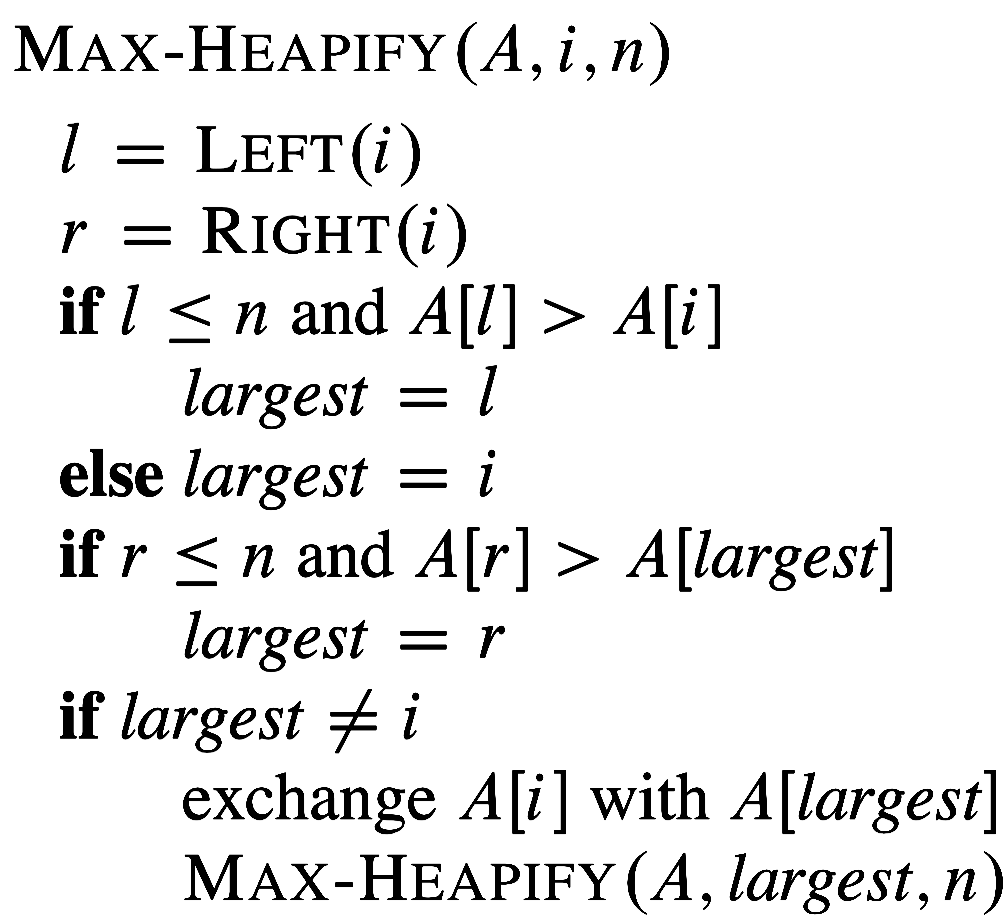
\includegraphics[width=0.7\linewidth]{images/heapify.png}
        \vspace{6pt}
        
        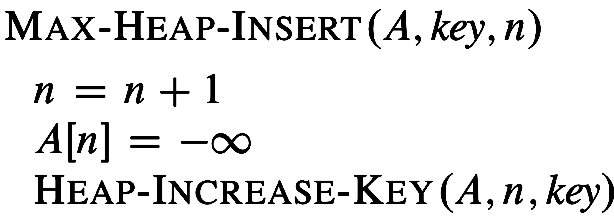
\includegraphics[width=0.7\linewidth]{images/heap-insert.png}
        \vspace{6pt}
        
        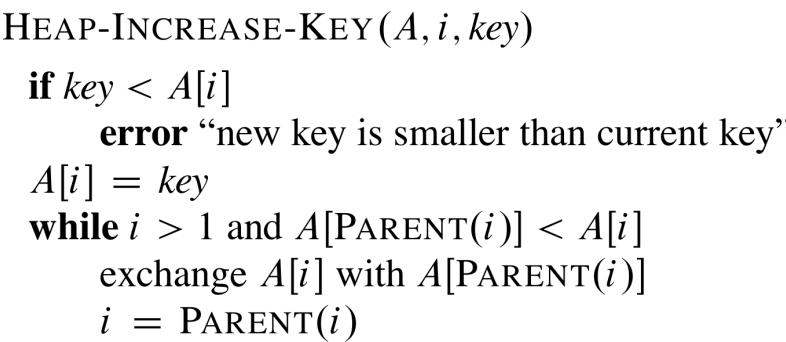
\includegraphics[width=0.7\linewidth]{images/heap-increase-key.png}
        \vspace{6pt}
        
        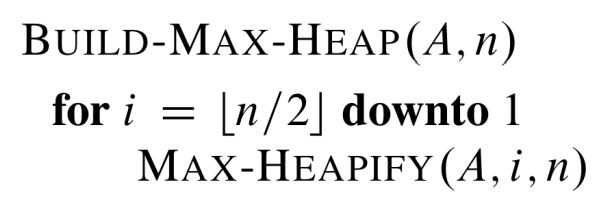
\includegraphics[width=0.7\linewidth]{images/build-max-heap.png}
        \vspace{6pt}
        
        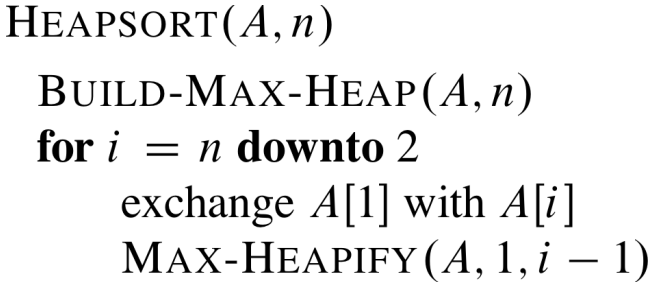
\includegraphics[width=0.7\linewidth]{images/heapsort.png}
    \end{minipage}
}} 